\documentclass{standalone}

\AtBeginDocument{\renewcommand{\AtBeginDocument}[1]{}}
\usepackage{siunitx}

\usepackage{pgfplots}
\pgfplotsset{compat=newest}


\begin{document}

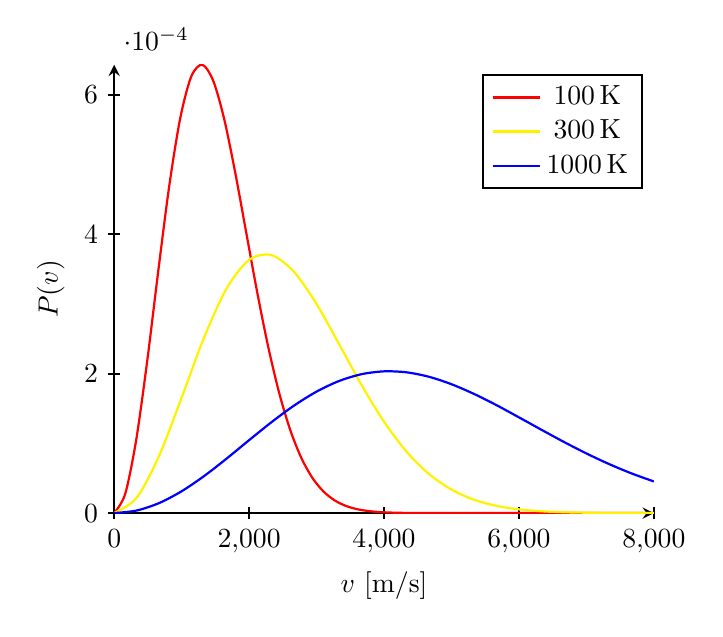
\begin{tikzpicture}

  \def\kB{1.3806488e-23}
  \def\m{1.660538921e-27}% atomic mass unit
  \def\w#1{4*pi*(\m/(2*pi*\kB*#1))^(3/2)*x^2*exp(-\m*x^2/(2*\kB*#1))}

  \begin{axis}[
    domain = 0:8000,
    xlabel = $v$ [\si{\metre\per\second]},
        ylabel = $P(v)$,
        smooth,
        thick,
        axis lines = left,
        every tick/.style = {thick}]

    \addplot[color=red,samples = 50]{\w{100}};

    \addplot[color=yellow]{\w{300}};

    \addplot[color=blue]{\w{1000}};

    \legend{\SI{100}{\kelvin},\SI{300}{\kelvin},\SI{1000}{\kelvin}}

  \end{axis}
\end{tikzpicture}

\end{document}